% LTeX: language=de-DE
\appendix
\chapter{Code Darstellungen}
\label{sec:code-darstellungen}

\inputminted{python}{{assets/code/main-api.py}}
\vspace*{-3mm}
\captionof{listing}{API\label{lst:api}}
\vspace*{3mm}

\inputminted{python}{{assets/code/driving_logic.py}}
\vspace*{-3mm}
\captionof{listing}{Driving Logic\label{lst:driving_logic}}
\vspace*{3mm}

\chapter{Darstellungen}
\label{sec:darstellungen}

\begin{figure}[H]
    \centering
    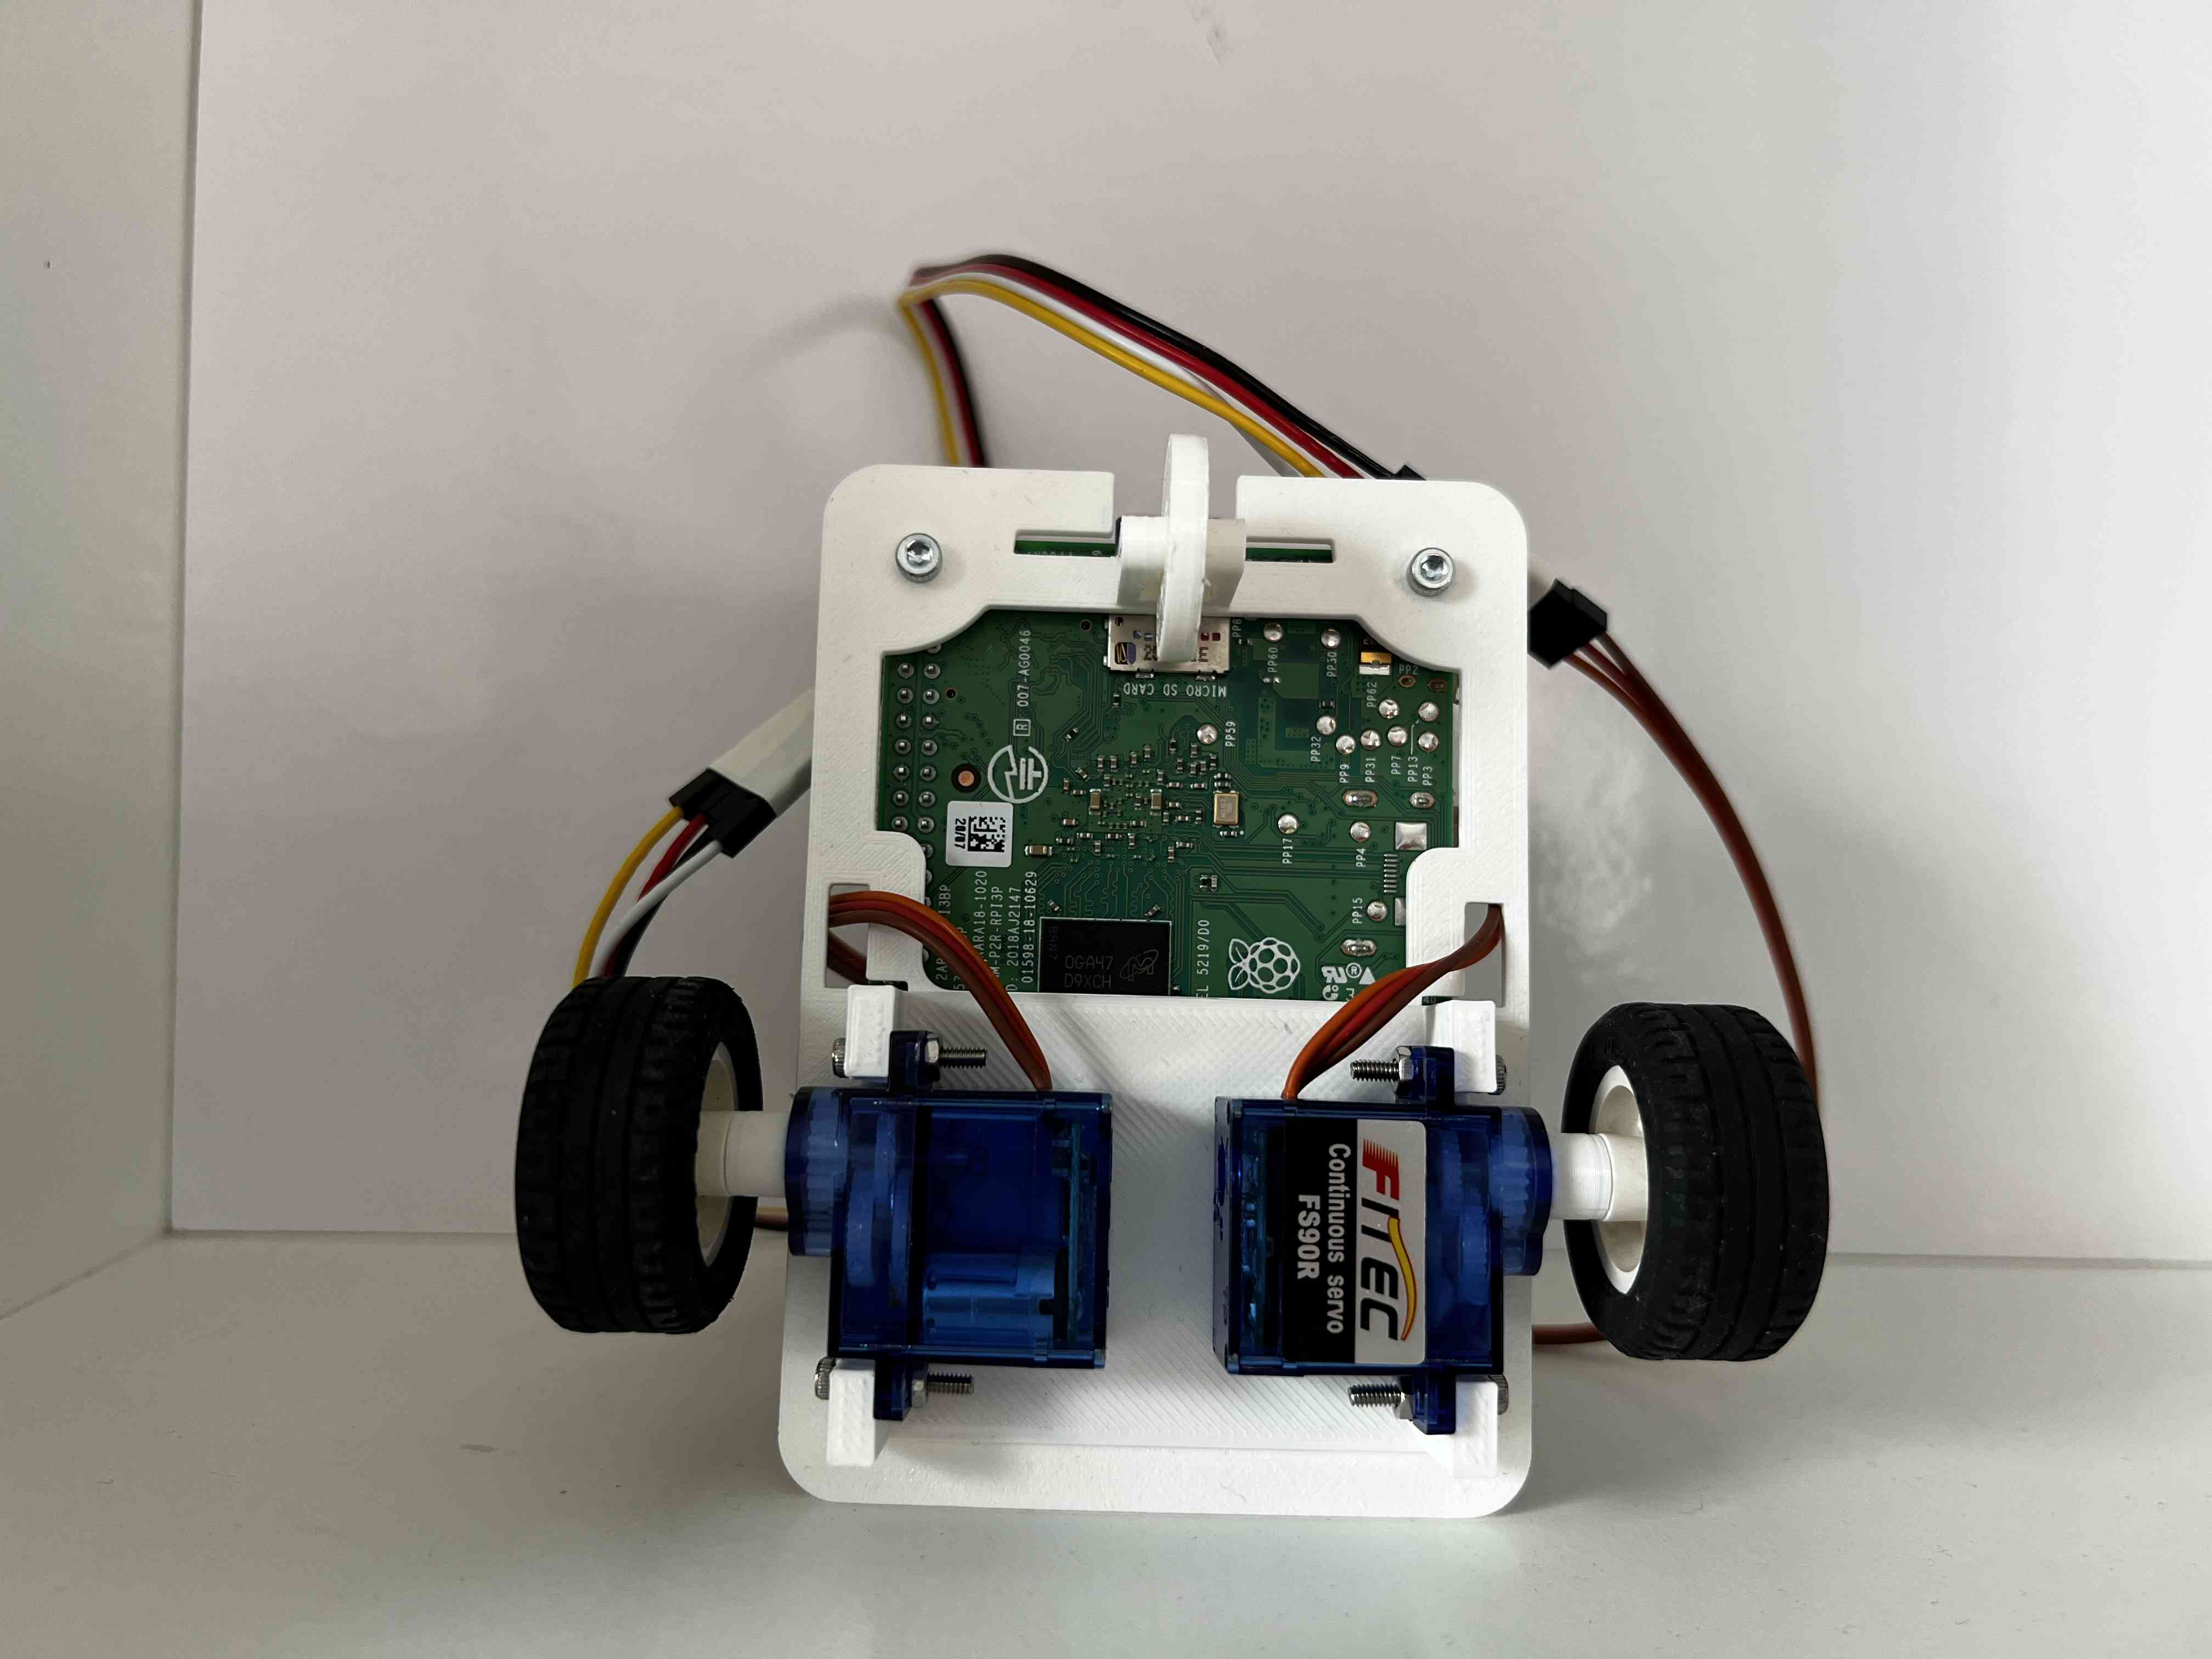
\includegraphics[width=\textwidth]{robot1.jpg}
    \caption{Ansicht von unten (groß)}
\end{figure}

\begin{figure}[H]
    \centering
    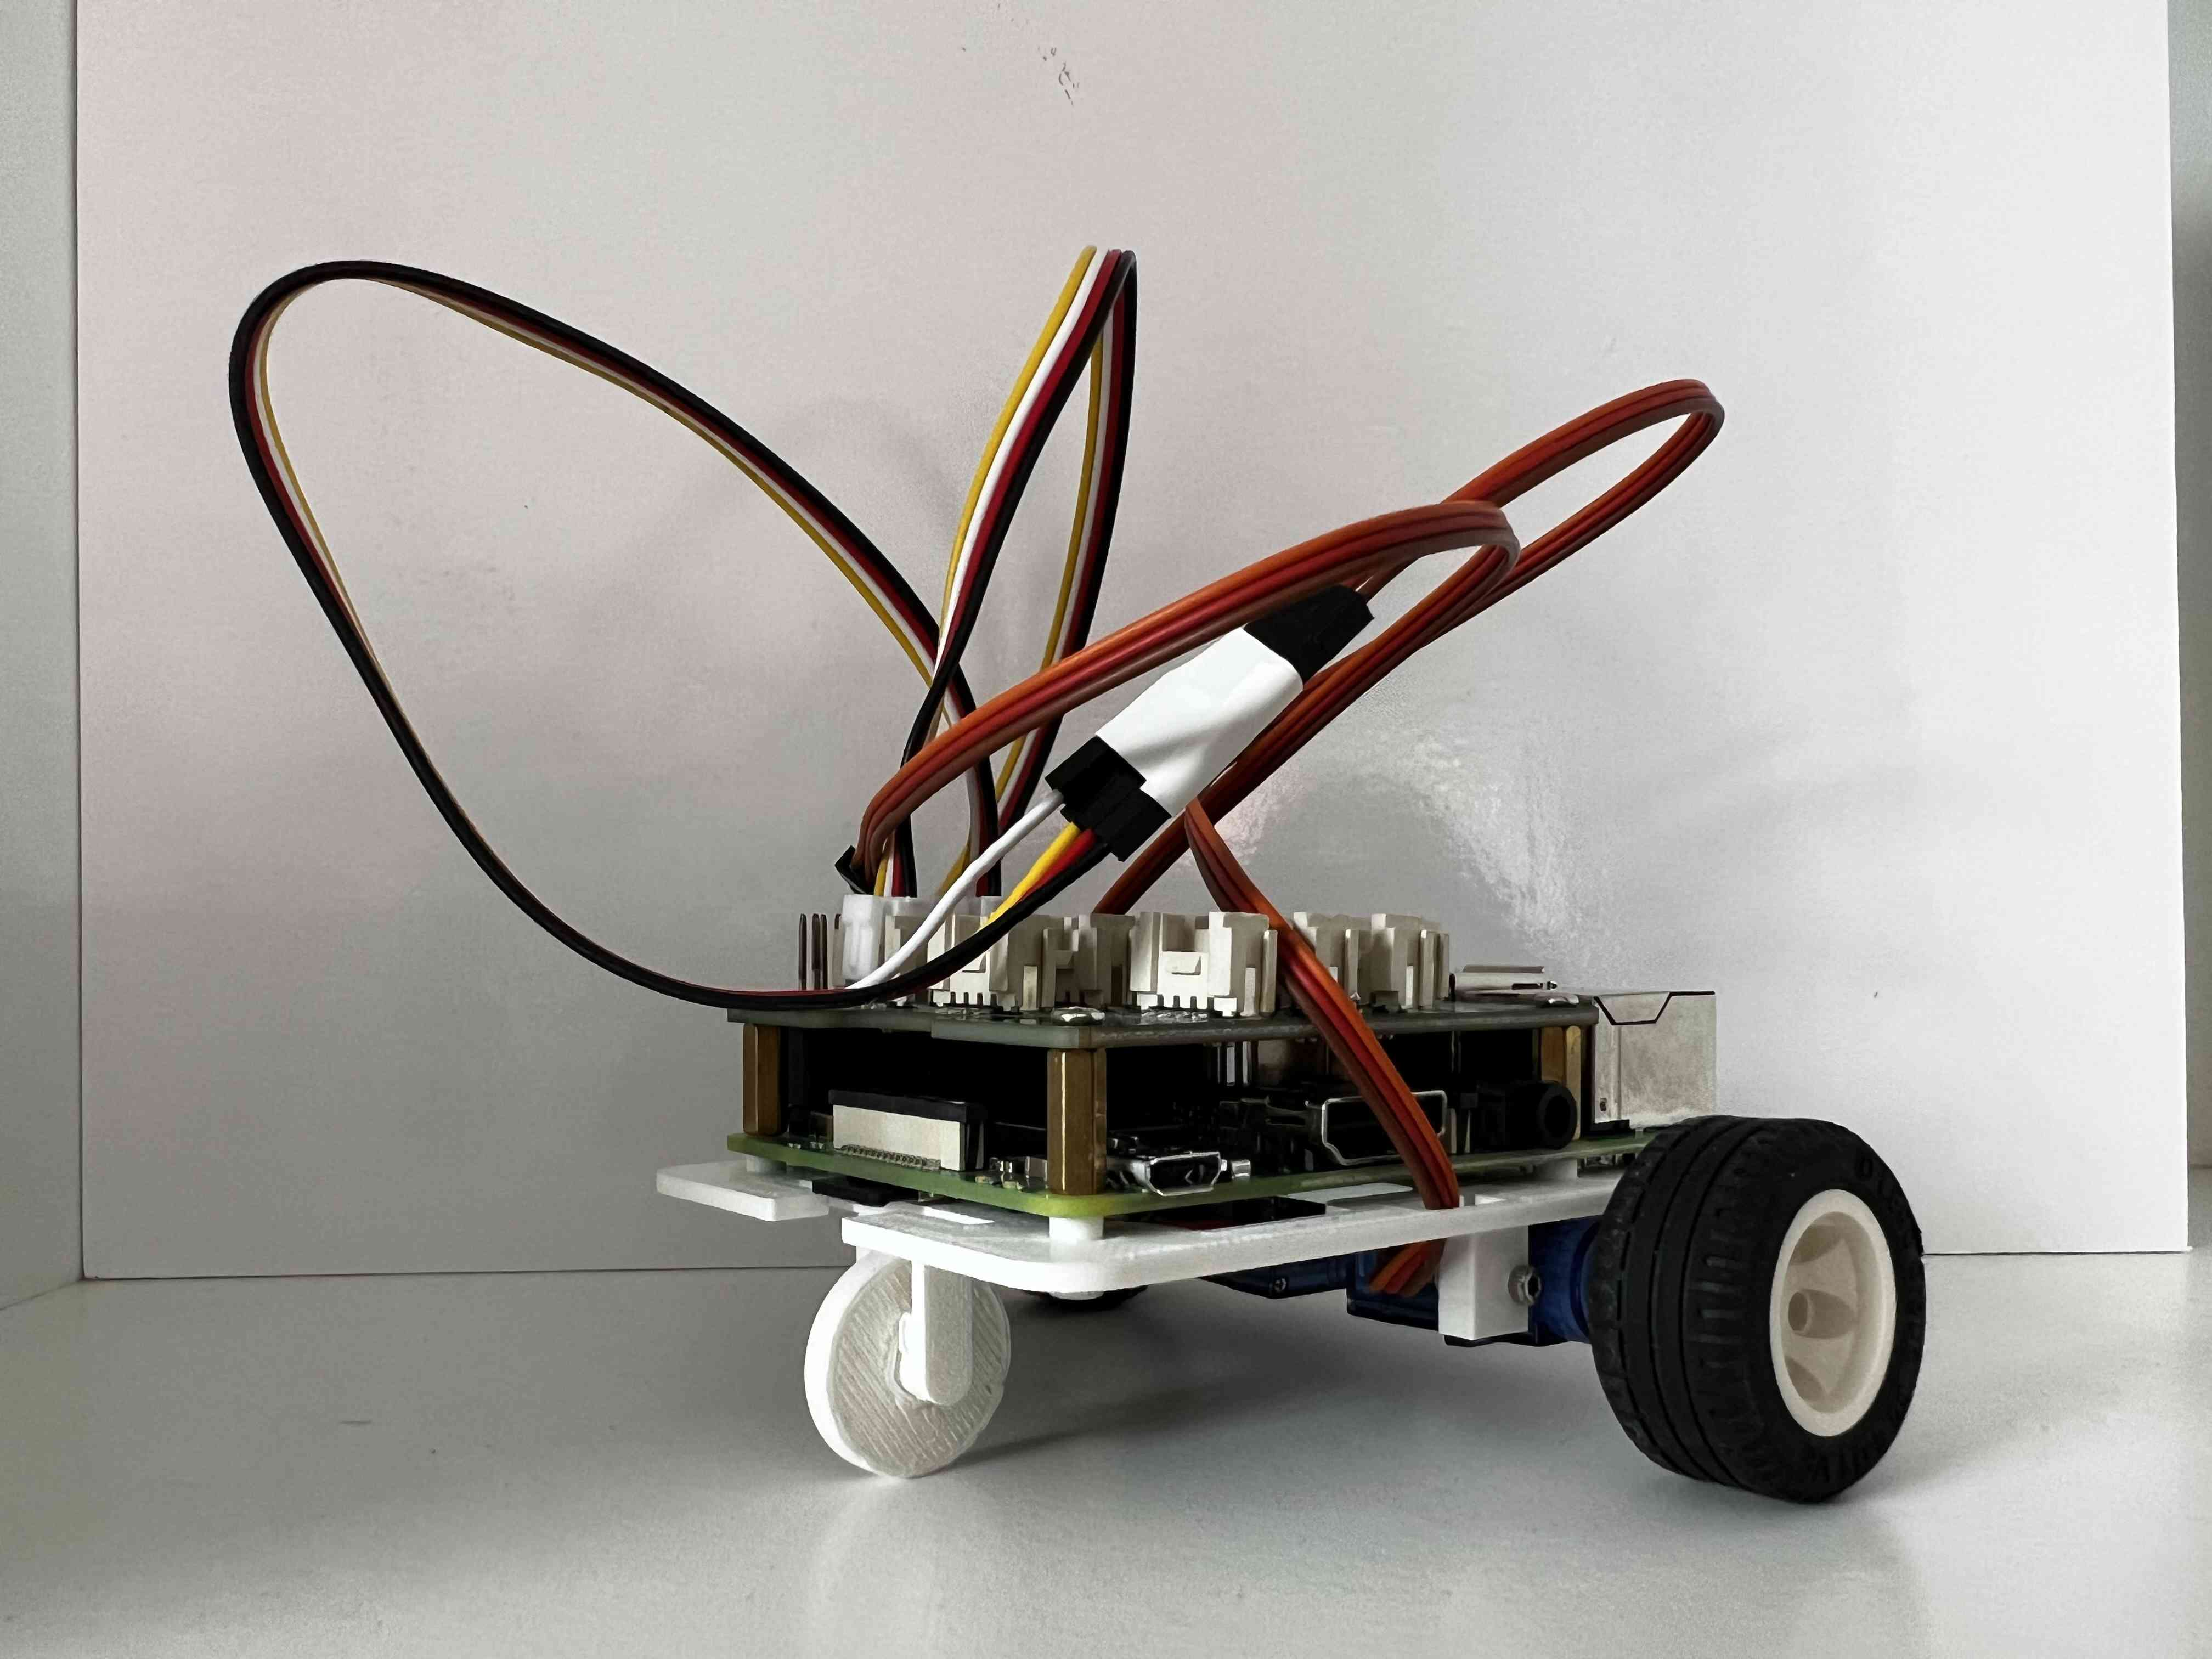
\includegraphics[width=\textwidth]{robot2.jpg}
    \caption{Seitenansicht (groß)}
\end{figure}
